\subsection{Multi-dimensional Profiling}
\label{sec:profiling}

The goal of our profiling stage is to explore the bandwidth-accuracy trade-off
and generate a \textit{profile} that is Pareto-optimal.

We first define terms and notations we will use. Each \texttt{maybe} operator
within an application corresponds to a knob $k$. Suppose the application has $n$
knobs, their combination forms a configuration $c = [k_{1}, k_{2},
... k_{n}]$. The set of all configurations $\mathbb{C}$ is the space that our
profiling system need to explore.

There are two mappings that we are particularly interested: a mapping from a
particular configuration to its bandwidth requirement $B(c)$ and the accuracy
measure $A(c)$. The Pareto-optimal set $\mathbb{P}$ can then be defined
(\autoref{eq:pareto}): for all $c \in \mathbb{P}$, there is no alternative
configuration $c'$ that requires less bandwidth while giving a higher accuracy.

{\small
\begin{equation}
  \mathbb{P} = \{ c \in \mathbb{C} : \{ c' \in \mathbb{C}: B(c') < B(c),
  A(c') > A(c) \} = \varnothing\}
  \label{eq:pareto}
\end{equation}
}%

\begin{table}
  \centering
  \begin{tabular}{r l}
    \toprule
    \textbf{Symbol} & \textbf{Description} \\
    \midrule
    $n$ & number of degradation operations \\
    $k_i$ & the \textit{i}-th degradation knob \\
    $c = [k_{1}, k_{2}, ... k_{n}]$ & one specific configuration \\
    $\mathbb{C}$ & the set of all configurations \\
    \midrule
    $B(c)$ & bandwidth requirement for $c$ \\
    $A(c)$ & accuracy measure for $c$ \\
    $\mathbb{P}$ & Pareto efficienct set \\
    \bottomrule
  \end{tabular}
  \caption{Notations used in profiling.}
  \label{tab:notations}
\end{table}

Since there is often no closed form relation for $B(c)$ and $A(c)$, our system
takes a data-driven approach: with a representative dataset and an
application-specific utility function, our system evaluates each configuration
for their bandwidth demand and accuracy degradation. The degradation could
either be measured against the groundtruth; or in the case when labelled dataset
is not available, the system uses the reference results when all degradations
are turned off.

\begin{figure}
  \centering
  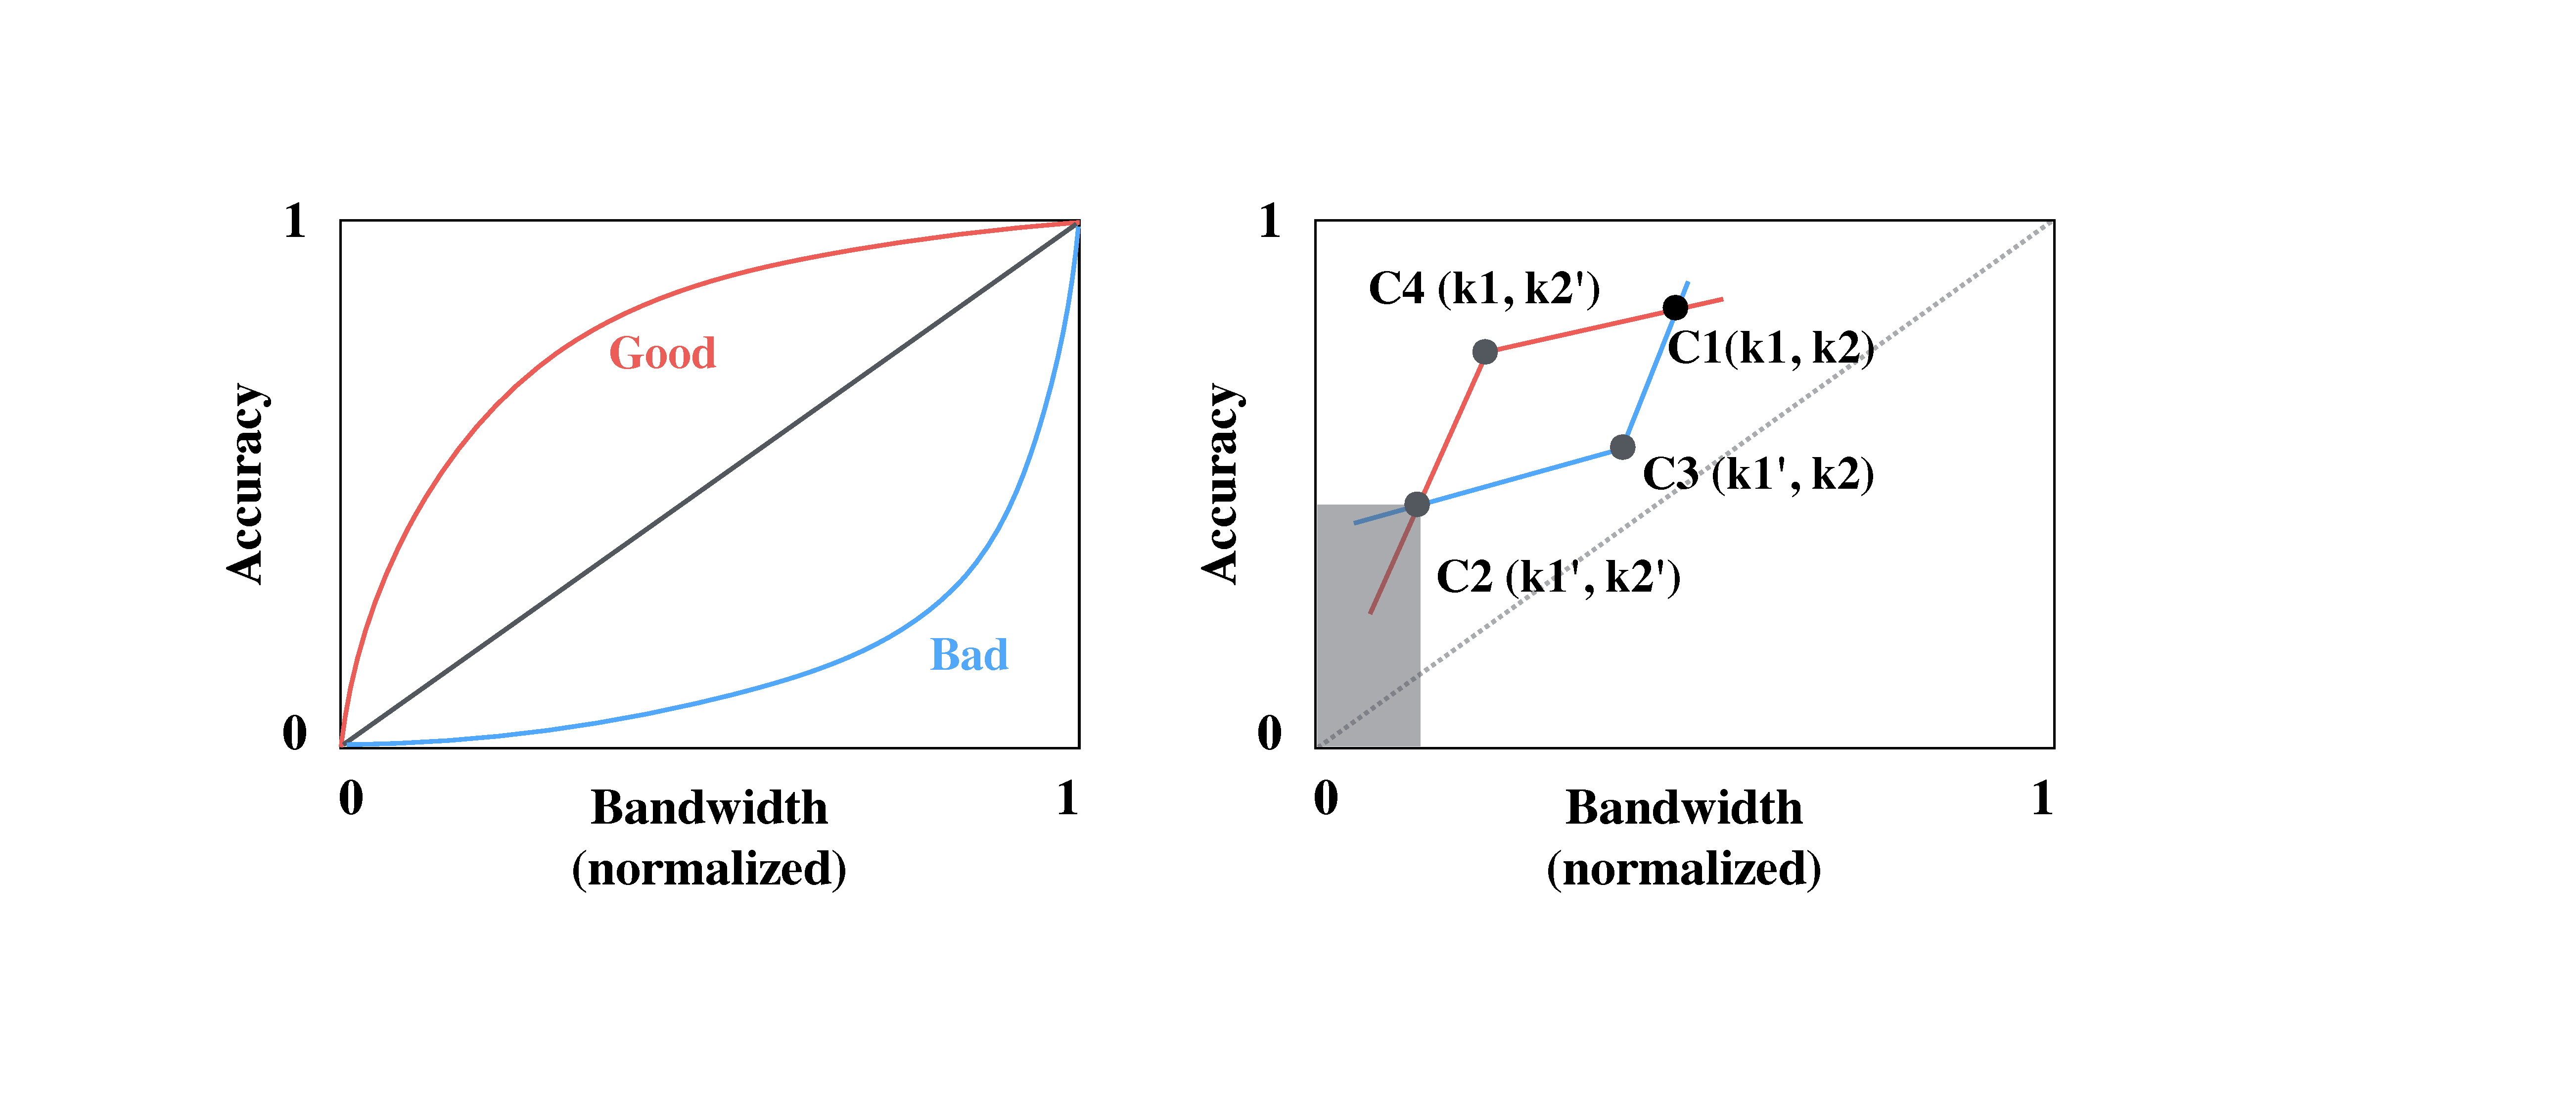
\includegraphics[width=\columnwidth]{figures/degrade.pdf}
  \caption{Illustration on the behavior of different degradation operations.}
  \label{fig:bat}
\end{figure}

When only one knob is involved, we can represent its impact using
bandwidth-accuracy curve (\autoref{fig:bat} left) and quantify the effect with
the area under the curve (AUC). Each curve consists of the point with coordinate
$(B(c), A(c))$ when configuration $c$ is used. The straight line from (0, 0) to
(1, 1) splits the space into two parts. If a degradation's profile lies above
this line, it indicates that this operation can be effective for the goal of
saving bandwidth while minimizing accuracy drop. For degradation operations
that's below the straight line, much of the data information is gone even at
minor bandwidth drop. The Pareto-optimal strategy is the profile that has a
maximal AUC.

While $B(c)$ and $A(c)$ can be monotonic along individual dimension. When
combined, it poses complex behavior. The right half illustrates
\autoref{fig:bat} illustrates it.

While the complexity prohibits further analytical analysis of the degradation
behavior, in practice, several techniques can make the problem tractable. First,
Exploring these configurations is an embarrassingly parallel task. The profiling
can be made trivially parallel. Besides, when the degradation level increases or
when multiple degradation operations are in effect, the amount of data as well
as the computational complexity are also dramatically reduced.  Moreover,
developers can specify a lower bound on the accuracy and the profiling can stop
searching the space that is worst than a known configuration (such as the gray
area in \autoref{fig:bat}).

%%% Local Variables:
%%% mode: latex
%%% TeX-master: "sigcomm2017"
%%% End:
